\section{Contributions}

\begin{figure}[h]
  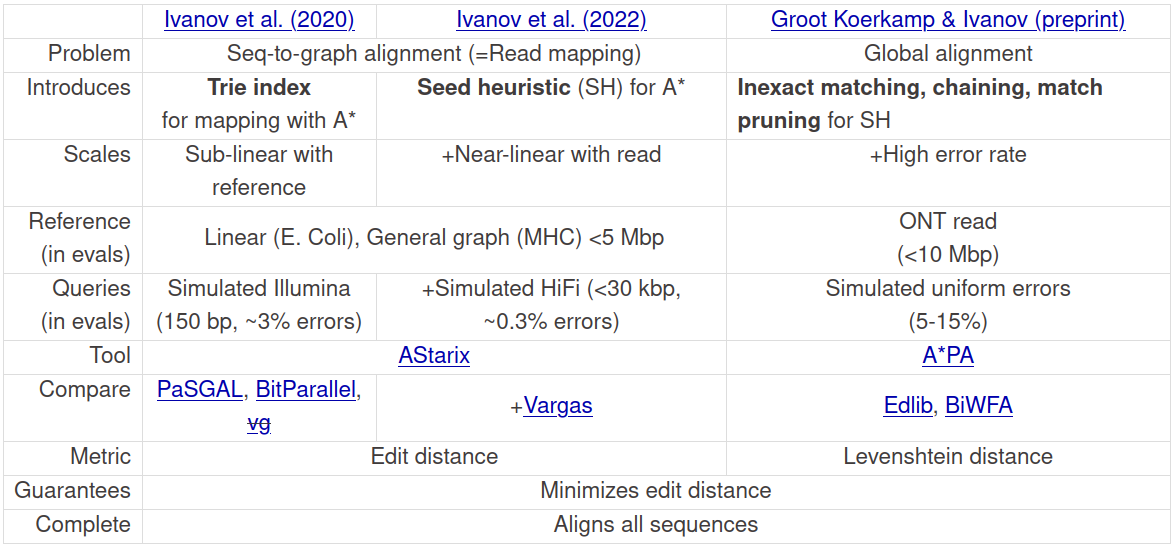
\includegraphics[width=1.0\linewidth]{media/ownpubs-table.png}
  \caption{Overview of the publications.}
  \label{tab:ownpubs}
\end{figure}

%\subsection{Knowledge gap}
\dictum{%
   Provably optimal and heuristically fast.}
\vskip 1em

We have effectively applied the \A algorithm to optimal sequence alignment. We
demontrated that the additional information from the whole sequence can improve
the scaling with query length, reference size and error rate, substantially
decrease the necessary computations, and result in algorithms that are orders of
magnitude faster than existing optimal algorithms. We apply the \A approach to
two types of alignment: semi-global (alignment) and global.

\subsection{Principled approach by shortest paths}
shortest paths,

A*, admissibility

\subsection{Optimality guarantees}
To ensure that our algorithms are practical, we introduce a number of
algorithmic optimizations which increase performance and decrease memory
footprint.

We also prove that all optimizations (greedy matching, ) are preserving the optimality.

\subsection{Scaling with reference size using a trie index}

\subsection{Scaling with query length using a seed heuristic}

\subsection{Scaling with error rate using inexact matching and chaining}

Informed search: Two-stage algorithm, similar to Aho-Corasick, increasingly more information (length, prefix, seeds, chaining seeds, chaining seeds + gaps)

\subsection{Aligning to general graph references}

\subsection{Implementations}

	
% trie
We present an algorithm for the \emph{optimal alignment} of sequences to
\emph{genome graphs}. It works by phrasing the edit distance minimization
task as finding a shortest path on an implicit alignment graph. To find a
shortest path, we instantiate the \A paradigm with a novel domain-specific
heuristic function that accounts for the upcoming subsequence in the query
to be aligned, resulting in a provably optimal alignment algorithm called
\astarix.

Experimental evaluation of \astarix shows that it is 1--2 orders of magnitude
faster than state-of-the-art optimal algorithms on the task of aligning Illumina
reads to reference genome graphs.

% seedh
We present a novel \A \emph{\seedh} that enables fast and optimal
sequence-to-graph alignment, guaranteed to minimize the edit distance of the
alignment assuming non-negative edit costs.

We phrase optimal alignment as a shortest path problem and solve it by
instantiating the \A~algorithm with our \seedh. The \seedh first extracts
non-overlapping substrings (\emph{seeds}) from the read, finds exact seed
\emph{matches} in the reference, marks preceding reference positions by
\emph{crumbs}, and uses the crumbs to direct the \A search. The key idea is to
punish paths for the absence of foreseeable seed matches. We prove admissibility
of the \seedh, thus guaranteeing alignment optimality.

Our implementation extends the free and open source aligner and demonstrates
that the \seedh outperforms all state-of-the-art optimal aligners including
\graphaligner, \vargas, \pasgal, and the \prefixh previously employed by
\astarix. Specifically, we achieve a consistent speedup of >60$\times$ on both
short Illumina reads and long HiFi reads (up to 25kbp, 0.3\% error rate), on
both the \textit{E.~coli} linear reference genome (1Mbp) and the MHC variant
graph (5Mbp). Our speedup is enabled by the \seedh consistently skipping
>99.99\% of the table cells that optimal aligners based on dynamic programming
compute.

% global
\paragraph{Methods}
We solve exact global pairwise alignment with respect to edit distance by using
the \A shortest path algorithm on the alignment graph. In order to efficiently
align long sequences with high error rate, we extend the \emph{seed~heuristic}
with \emph{match~chaining}, \emph{inexact~matches}, and the novel
\emph{match~pruning} optimization. We prove the correctness of our algorithm and
provide an efficient implementation in \astarpa.
\paragraph{Results}
We evaluate \astarpa on synthetic data (random sequences of length $n$ with
uniform errors with rate $e$) and on real long ONT reads of human data. On the
synthetic data with $e{=}5\%$ and $n{\leq}10^7\bp$, \astarpa exhibits a
near-linear empirical runtime scaling of $n^{1.08}$ and achieves ${>}250\times$
speedup compared to the leading exact aligners \edlib and \wfa. Even for a high
error rate of $e{=}15\%$, the empirical scaling is $n^{1.28}$ for
$n{\leq}10^7\bp$. On two real datasets, \astarpa is the fastest aligner for
$58\%$ of the alignments when the reads contain only sequencing errors, and for
$17\%$ of the alignments when the reads also include biological variation.